%%% File encoding: UTF-8
%%% äöüÄÖÜß  <-- no German umlauts here? Use an UTF-8 compatible editor!

%%% Magic comments for setting the correct parameters in compatible IDEs
% !TeX encoding = utf8
% !TeX program = pdflatex 
% !TeX spellcheck = de_DE
% !BIB program = biber

\documentclass[bachelor,english,smartquotes]{hgbthesis}
% Valid options in [..]: 
%    Type of work: 'diploma', 'master' (default), 'bachelor', 'internship' 
%		 Additionally for a thesis exposé: 'proposal (for 'bachelor' and 'master')
%    Main language: 'german' (default), 'english'
%    Turn on smart quote handling: 'smartquotes'
%    APA bibliography style: 'apa'
%%%-----------------------------------------------------------------------------

\RequirePackage[utf8]{inputenc} % Remove when using lualatex or xelatex!

\graphicspath{{images/}}  % Location of images and graphics
\logofile{logo}          % Logo file: images/logo.pdf (no logo: \logofile{})
\bibliography{references} % Biblatex bibliography file (references.bib)

%%%-----------------------------------------------------------------------------
\begin{document}
%%%-----------------------------------------------------------------------------

%%%-----------------------------------------------------------------------------
% Title page entries
%%%-----------------------------------------------------------------------------

\title{Predicting the activity of protein-ligand complexes}
\author{Lukas Fallmann}
\programname{Medizin- und Bioinformatik}

%\programtype{Fachhochschul-Bachelorstudiengang} % select/edit
\programtype{Fachhochschul-Bachelorstudiengang}


\placeofstudy{Hagenberg}
\dateofsubmission{2023}{06}{27} % {YYYY}{MM}{DD}

\advisor{Micha Johannes Birklbauer, M.Sc.} % optional

%\strictlicense % restrictive license instead of Creative Commons (discouraged!)

%%%-----------------------------------------------------------------------------
\frontmatter                                   % Front part (roman page numbers)
%%%-----------------------------------------------------------------------------

\maketitle
\tableofcontents

\chapter{Preface}






 % A preface is optional
\chapter{Abstract}


This should be a 1-page (maximum) summary of your work in English.

		
\chapter{Kurzfassung}

\begin{german}
An dieser Stelle steht eine Zusammenfassung der Arbeit, Umfang
max.\ 1 Seite. 
...
\end{german}			

%%%-----------------------------------------------------------------------------
\mainmatter                                    % Main part (arabic page numbers)
%%%-----------------------------------------------------------------------------

\chapter{Introduction}
\label{cha:Introduction}



\section {Overview of the topic}
\section {Why is it important}
\section {What are current methods that are prominently used}
\section {Machine Learning in drug design / activity prediction}
\section {Interactions}
\section {Goals}


\chapter{Methods}
\label{cha:Methods}


\section{Data description}

The following chapter is dedicated to explaining the data used for this thesis.
This includes detailed descriptions of the protein complexes as well as their interaction types.

\subsection{Proteins}
The following five proteins have been used to conclude this thesis:
\subsubsection*{Acetylcholinesterase}
Acetylcholinesterase (AChE) is an efficient enzyme in the nervous system that breaks down 
acetylcholine (Ach), a messaging molecule, into choline and acetate. 
It's found in high concentrations at junctions between nerve cells and muscles.
AChE has various functions beyond just breaking down Ach, 
and it's present in both nerve and non-nerve tissues.
Because AChE is so important, some toxins like insecticides and nerve agents target it.
 This versatility of AChE makes it a key player in nervous system function
 and a potential target for drugs to treat diseases\cite[]{Tripathi2010}.
\subsubsection*{Cyclooxygenase 1}
Cyclooxygenase 1 (COX1) and its isoform Cyclooxygenase 2 (COX2) play a substantial role in 
synthesising various prostaglandins. Due to their linkage with inflammations and pain
COX molecules are often targeted by anti-inflammatory drugs. In contrast to COX2, COX1 is found in most tissues
across the body. In addition to that COX1 is largely attributed with homeostatic functions
such as hemostasis and gastric cytoprotection\cite[]{Rouzer2009}.
\subsubsection*{Dipeptidyl peptidase IV}
Dipeptidyl peptidase IV(DPP4) can be is partially responsible
for hydrolysis of a prolyl bond between two residues from the N-terminus.
DPP4 is present in several processes including metabolism and cancer biology.
Due to its role within the metabolism DPP4 inhibitory drugs have been successfully used in the treatment of diseases type two.
DPP4 also plays a substantial role in the diagnosis of certain types of cancer. 
In most cases DPP4 is up regulated near cancerous growth, therefore locally elevated DPP4 levels can be 
an indicator for cancer\cite[]{Yu2010}.
\subsubsection*{Monoamine oxidase B}
Monoamine oxidase B(MAOB) plays a major role in the breakdown of neurotransmitters(monoamines) within the body.
The compound is mainly expressed in glial-cells and platelets.
Its function categorizes MAOB as an important research compound, as MAOB inhibition has been proven to improve 
various neurological conditions. This stems from the fact that changes in the monoamine levels are
associated with a myriad of neurological problems\cite[]{Ramsay2016}.
\subsubsection*{Soluble epoxide hydrolase}
Soluble epoxide hydrolase (sEH) is part of an inflammatory pathway similar to COX.
It has been shown that inhibition of sEH reduces inflammation. In contrast to COX it does not 
completely disable the synthesis of pro-inflammatory compounds but rather balance their levels\cite[]{Schmelzer2005}.
\subsection{Interactions → !WIP! ask Micha regarding grade of detail}
The following interactions have been chosen for this thesis:

\begin{table}[h!]
    \centering
\begin{tabular}{ | m{10em} | m{30em}| } 
    \hline
    \textbf{interaction} &\textbf{description\cite[]{Birklbauer2021}}
    \\
    \hline
    hydrogen bonds& A hydrogen bond is defined as the interaction between a 
    hydrogen atom, connected to a more electronegative atom, and another atom or molecule. \\
    \hline
    water bridges   &A water bridge occurs when the ligand and the protein
    both bind to a water molecule through hydrogen bonds.\\
    \hline
    salt bridges&  Salt bridges are ion pairs which stick together due to
    large difference in charge and the resulting electrostatic interaction. \\
    \hline
    halogen bonds&  Halogen bonds are defined as the interactions between the electrophilic region
    around a halogen atom and a nucleophilic region.\\
    \hline
    hydrophobic interactions& Aggregates formed as a result
    of a hydrophobic interaction between hydrocarbons in an 
    aqueous medium are called hydrophobic interactions.\\
    \hline
    pi-stacking   & Interactions between neighboring aromatic 
    rings are called pi-stacking. Due to the pi-electron density the ring is partially positively charged around 
    the periphery and negatively charged above both aromatic faces. As a result electrostatic forces build between aromatic rings,
     and they are attracted to one another.\\
    \hline
    pi-cation& Cations and pi-stacks who bind through electrostatic 
    forces at pi-stacks face are called pi-cation interactions.\\
    \hline
   \end{tabular}
   \caption{interaction types}
\end{table}
    


\subsection{Data origin and structure}
The provided data is a byproduct of the thesis \cite[]{Birklbauer2021} by Micha Birklbauer.
The interaction data was produced using the \textit{PLIP Algorithm} \cite[]{Salentin2015} 
on the aforementioned proteins.

The PLIP Algorithm consists of four major stages: 
\begin{description}
    \item[Structural Preparation] -- \textbf{SP} 
    \newline During the preparation step the input structure is hydrogenated and the ligands(including their binding sites) are extracted. 
    \item[Functional Characterization] -- \textbf{FC}
    \newline Using the structure of the complex a myriad of functional groups are detected. This includes binding site atoms, hydrophobic atoms and aromatic rings just to name a few.
    \item[Rule Based Matching] -- \textbf{RBM}
    \newline In the third step the algorithm investigates all interactions between the ligand and the protein, which can be attributed to geometric constraints. Hydrogen bonds are detected here.
    \item[Filtering of Interactions] -- \textbf{FoI}
    \newline This is a cleanup step where redundant or overlapping interactions get removed from the dataset. 
\end{description}
\newblock
The result of the PLIP Algorithm is a lineup of every interaction for each binding site and ligand\cite[]{Salentin2015}.
This data has been used as a basis for the machine learning approaches discussed in this thesis.

\section{Data partitioning}
To validate the results of training various machine learning methods the provided data concerning
the five targets was split into a training-set as well as a test-set. To achieve a 70/30 train/test split ratio each sample was randomly assigned 
to one of the two datasets\cite[]{Xu2018}.

In order to validate the machine learning approaches during training 10-fold cross-validation has been applied.
For the process of cross-validation the training dataset is split into $n$ equally large subsets.
The type of cross-validation implemented in this thesis uses all but one of these partitions to train the classification model and validates the 
results with the remaining partition. This process is repeated for all possible validation partitions\cite[]{Molinaro2005}.

\section{Machine-Learning approaches !WIP!}
The following chapter aims to explain the basic machine learning approaches used for this thesis.


\subsection{Neural networks}
The practical neural network approach of this thesis has been implemented using the Tensorflow\cite[]{Abadi2016} library.
\label{cha:nn}

\subsection{K nearest neighbor}
\label{cha:knn}
\acrfull*[]{knn} is a very simple classification algorithm for the numerical features used in this thesis.
First, the source dataset is converted into a vector representation. Each sample of the source dataset is represented as and $n$-dimensional vector, where $n$ is the amount
of features within that particular dataset. In addition to that vector the class of each sample is also saved.
The classification is achieved by representing a new sample within the aforementioned vector-space.
For the new sample the $k$ nearest neighbors are calculated using a distance metric, where $k$ is an odd-number. For this thesis the \textit{euclidean} distance was used.
The euclidean distance for two vectors($\mathrm{v}_{1},\mathrm{v}_{1}$) in the $n$ dimensional space is defined as follows:
\begin{equation*}
    euclidian(\mathrm{v}_{1},\mathrm{v}_{1}) = \sqrt[]{\sum_{i=1}^{n} (\mathrm{v}_{1,i} -\mathrm{v}_{2,i})^2} 
\end{equation*}
In the base version of \acrshort*[]{knn} the new sample is put in the same class as the majority of its $k$-neighbors.
In addition to that the $k$ nearest neighbors can also be weighted using their distance to the new sample\cite[]{Cunningham2022}. 

K nearest neighbor for this thesis has been implemented using the \href{https://scikit-learn.org/stable/index.html}{scikit-learn package}. 

\subsection{Random forest}
\label{cha:rf}
In the following the base concept of the random forest algorithm used for this thesis will be explained.
\\The random forest algorithm is a collection of identically distributed decision trees\cite[]{Breiman2001}.
The algorithm can be split into the creation of a bootstrapped dataset, the creation of decision trees and the evaluation of said trees.

\subsubsection*{Bootstrapping}
The goal of this step is to create a new dataset for each decision tree. This happens by randomly selecting 
samples from the source dataset. It is noteworthy that samples can be selected multiple times when creating such a bootstrapped dataset.
Furthermore, not all samples are included in each dataset. Those samples, which are not included in any dataset are called \textit{out-of-bag} samples 
and are later used for further tree enhancement. With those bootstrapped dataset decision trees can be built in the next step.

\subsubsection*{Creation of decision trees}
For each bootstrapped dataset a new decision tree is created using the following steps. Firstly a number of features is randomly selected.
For those selected features it is determined, which feature is best for splitting the data, so that the classes are separated very clearly.
This is usually determined using the \textit{Gini}-impurity.
The Gini-impurity is a measure of how well a dataset can be divided using a certain feature.

The Gini-impurity can be calculated at each node of a decision-tree and is ranged from 0 to 0.5.
Let $k$ be the number of classes and let $\mathrm{p}_{i}$ be the probability of a sample belonging to the class($i$) and the Gini-impurity($Gini(D)$) of the dataset($D$)
at a certain node within the tree can be defined as follows:
\begin{equation*}
    Gini(D) = 1 - \sum_{i=1}^{k} \mathrm{p}_{i}^2
\end{equation*} \cite[]{Karabiber}

After selecting the splitting feature the data is split and the whole process repeats for the newly created nodes.
When selecting a new splitting feature all features already existing in the tree can be used again. This whole process is 
repeated until every path of the tree leads to a clear classification result\cite[]{Breiman2001}.

\subsubsection*{Evaluation and optimization}
After the construction of the forest the performance can be evaluated using the out-of-bag samples.
This is achieved by classifying the samples from the out-of-bag dataset using the random-forest. Each tree within the forest is provided with the data from the sample
and votes for a class based on the samples features.

The parameters of a random forest, for example the number of features considered at each node, can be optimized. To achieve that multiple forests with 
different parameters are generated and the best performing one for the out-of-bag samples is selected\cite[]{Breiman2001}.

For this paper the random forest approach has been implemented using the \href{https://scikit-learn.org/stable/index.html}{scikit-learn package}. 





\section{Quality metrics}
In order to make the results from this thesis comparable to the results from the 
scoring function introduced in \cite[]{Birklbauer2021} by Micha Birklbauer the same quality metrics have been 
implemented for this thesis. The following will provide an overview for the used metrics.
\subsection{Terminology} \label{terminology}
To calculate the metrics that are mentioned within this chapter the following base terms are necessary:
\begin{description}
    \item [TP] -- \textbf{T}rue \textbf{P}ositives are active samples, which are classified as such
    \item [TN] -- \textbf{T}rue \textbf{N}egatives are inactive samples, which are classified as such
    \item [FP] -- \textbf{F}alse \textbf{P}ositives are inactive samples, which are classified as active
    \item [FN] -- \textbf{F}alse \textbf{N}egatives are active samples, which are classified as inactive 
\end{description}

\subsection{Visual metrics}
For better visualization of the four base metrics mentioned in \href{terminology}{2.4.1}
this thesis displays the resulting data in a confusion matrix. This metric displays distribution of the results over the four base metrics.

In addition to that, the ROC(receiver operating characteristic) curve will also be displayed for the results.
The ROC curve is a collection of points in a two-dimensional 
space, where their location is defined by the FPR \href{fpr}{2.4.4} on the x-axis and the TPR($\frac{\#TP}{\#TP+\#FN}$) on the y-axis. 
Each point on this line depicts the ratio of FPR to TPR at a certain score cutoff. \cite[]{Lopes2017}


\subsection{Accuracy}
\acrfull*[]{acc} describes which portion of the predicted samples was accurately assigned to the correct class and is defined as follows:
\begin{equation*}
    \text{ACC} = \frac{\#TP+\#TN}{\#TP+\#TN+\#FP+\#FN}
\end{equation*}
\cite[]{Hossin2015}
\subsection{False positive Rate}\label{fpr}
\acrfull*[]{fpr} describes the compounds that were incorrectly classified as active in relation to all inactive compounds and is defined as follows:
\begin{equation*}
    \text{FPR} = \frac{\#FP}{\#TN+\#FP}
\end{equation*}
\cite[]{Lopes2017}
\subsection{Area under the curve}
\acrfull*[]{auc} is a metric which stems from the ROC curve. 
The integral of the ROC curve is calculated using the \href{https://scikit-learn.org/stable/index.html}{scikit-learn}
 package and is always between 0 and 1\cite[]{Lopes2017}.
\subsection{Yield of Actives}
\acrfull*[]{ya} describes the true positive compounds in relation to all as active labeled compounds and is defined as follows:
\begin{equation*}
    \text{Ya} = \frac{\#TP}{\#TP+\#FP}
\end{equation*}
\cite[]{Giordano2022}
\subsection{Enrichment Factor}
The \acrfull*[]{ef} describes the relation of the truly active compounds among all as active predicted complexes and the relative share of active compounds in the dataset.
This metric is defined as follows:
\begin{equation*}
    \text{EF} = \frac{\frac{\#TP}{\#TP+\#FP}}{\frac{\#TP+\#FN}{\#TP+\#TN+\#FP+\#FN}}
\end{equation*}
\cite[]{Lopes2017}  
\subsection{Relative Enrichment Factor}
The \acrfull*[]{ref} describes the relation of the EF to the maximum achievable EF. The REF is defined as follows:
\begin{equation*}
    \text{REF} = \frac{100 *\#TP}{\min(\#TP + \#FP,\#TP+\#FN)}
\end{equation*} 
\cite[]{Lopes2017}  



\section{Feature engineering}
Feature engineering is the process of manipulating the given features within a dataset with the goal of improving the performance of
numerous machine learning techniques applied to the manipulated data. The following chapter explains the various methods that have been used
for this thesis.

\subsection{Feature engineering using random forest}
Due to the nature of the random forest algorithm, explained in \ref{cha:rf}, it can be used effectively to determine the most important
features within a dataset.
This section introduces the two feature engineering components within this thesis that are based on the random forest algorithm.
\subsubsection*{\acrfull*[]{mdi}}
The importance of each feature in a random forest is decided by how well a certain feature can divide the samples in to the desired groups.
The mean decrease in impurity is a measure designed to indicate this importance.
To calculate it the \textit{Gini}-impurity is needed. The Gini-impurity is a measure of how well a dataset can be divided using a certain feature.
The Gini-impurity can be calculated at each node of a decision-tree and is ranged from 0 to 0.5.
Let $k$ be the number of classes and let $\mathrm{p}_{i}$ be the probability of a sample belonging to the class($i$) and the Gini-impurity($Gini(D)$) of the dataset($D$)
at a certain node within the tree can be defined as follows:
\begin{equation*}
    Gini(D) = 1 - \sum_{i=1}^{k} \mathrm{p}_{i}^2
\end{equation*} \cite[]{Karabiber}

With that in mind the mean decrease in impurity can be calculated with the following steps.
At first the initial Gini-impurity needs to be calculated using the formula above with the classes \textit{active} and \textit{inactive}.
In a second step it is necessary to calculate the \textit{weighted Gini} after a split by a feature for each feature.
This is achieved by multiplying the relative amount of actives with the Gini-impurity of a given feature for an active classification. This is repeated for
the inactive component. Those two numbers combined equate the weighted Gini for that feature.
The average of the weighted Gini over all features equates to the mean decrease in impurity.
Let $\mathrm{g}_{f}$ be the weighted Gini for a feature($f$) and $n$ be the number of features then the mean decrease in impurity($mdi$) can be defined as follows:
\begin{equation*}
    mdi = \frac{1}{n} * \sum_{f=1}^{n} \mathrm{g}_{f}
\end{equation*}
With this metric the features with larger $\mathrm{g}_{f}$ are deemed the most crucial for classification\cite[]{Soman2023}.

In the following, results with the \textit{fe\_rf\_mdi}-prefix where calculated using this method.

\subsubsection*{Permutation importance}
Permutation importance is a feature engineering technique used to determine the most important features for classification within a tabular dataset.
At first a reference score($s$) is calculated using a random forest classifier. In the following step a feature column is randomly permutated.
After this \textit{corruption} of the source dataset the score is calculated again and compared to the reference score. This step can be repeated $K$ times in order
to improve its statistical viability. This process is repeated for all features.

Let $j$ be the feature, $K$ the repetitions per feature and $\mathrm{s}_{k,j}$ the score of each corrupted dataset, and the importance of each
feature($\mathrm{i}_{j}$) can be calculated as follows:
\begin{equation*}
    \mathrm{i}_{j} = s -\frac{1}{K}*\sum_{k=1}^{K} \mathrm{s}_{k,j}
\end{equation*}
If a feature is of greater significance to the model then the score will deviate greater from the reference value\cite[]{permutation_importance}.

This method is not particularly dependent on the random forest algorithm. The random forest classifier component can be substituted with any other classifier.

In the following, results with the \textit{fe\_rf\_per}-prefix where calculated using this method.

\subsection{Physical properties}
Feature engineering can also be based on meta-information concerning the provided datasets.
For this thesis two methods are proposed to enhance the data by removing possible \textit{noise-features} with the use of additional
knowledge concerning the datasets.
\subsubsection*{Selection of most frequent interactions}
To prevent overfitting the forty features(binding-sites) with the most interactions have been selected.
By removing the less occurring features the overall performance especially on the validation- and test-runs should improve.
Due to the reduction in the amount of features overfitting can be reduced, and the machine learning models are less distracted by
"unimportant" features.

In the following, results with the \textit{fe\_freq}-prefix where calculated using this method.

\subsubsection*{Removal of all hydrophobic interactions}
Of all, for this thesis considered interactions, hydrophobic interactions are generally the most frequent\cite[]{Freitas2017}. Therefore, it is of interest to reduce the overall
amount of features by removing all the hydrophobic interactions from the datasets in order to achieve more granular results.

In the following, results with the \textit{fe\_nonhydrop}-prefix where calculated using this method.

\subsection{\acrfull*[]{pca}}
Principal component analysis is a feature engineering method which aims to reduce the noise within a dataset, as well as maximize the amount of variance.
PCA works by representing the original dataset as through linear uncorrelated variables or components.
This is done in three steps:
\begin{enumerate}
    \item Restructuring of the data so that the data is represented as a $m \times n$ matrix where $m$ is the number of features and $n$ the number of samples.
    \item Subtract off the mean for each feature.
    \item Calculation of the principal components using \acrfull*[]{svd}.
\end{enumerate}
While the first two steps are quite clear, the third step will be explained in the following.

First the \acrshort*[]{svd} of the dataset needs to be defined.
\begin{equation*}
    X = U \cdot \Sigma \cdot V^T
\end{equation*}
Where $X$ is the original data matrix, $U$ is the matrix containing the eigenvectors of $X \cdot X^T$, $\Sigma$ contains the square-roots of the
eigenvectors of $X^T \cdot X$ and $V$ contains the eigenvectors of $X^T \cdot X$.

To get the transformed data it is necessary to multiply the $U$ matrix with $\Sigma$. 
The resulting projections are sorted according to variance\cite[]{Shlens2014}.

In the following, results with the \textit{fe\_pca}-prefix where calculated using this method.
\subsection{Balancing classes}
The data used for this thesis is not balanced, as there are more \textit{inactive} samples than \textit{inactives}.

Synthetic minority over-sampling(\acrshort*[]{smote}) can be used to balance the provided datasets. The aim of this technique is to synthetically 
generate samples from the minority class to balance the class distribution.
The \acrshort*[]{smote} algorithm starts by selecting a sample from the minority class and finding its $k$ nearest neighbors within that class.
For each of the selected neighbors the difference to the original sample is calculated. The differences are then scaled with a random factor 
between 0 and 1. Those scaled values are added to the original sample in order to create new samples.
This whole process is repeated for the unbalanced dataset until all classes are equally represented\cite[]{Chawla2002}.

In the following, results with the \textit{fe\_smote}-prefix where calculated using this method.


\chapter{Results}
\label{cha:Results}
The following chapter describes the results from the different machine learning approaches and the applied 
feature engineering techniques described in \href{cha:Methods}{Methods}.
\section{Feature Engineering Results for \acrshort*[]{ache}}
To evaluate different feature engineering approaches the protein \textit{Acetylcholinesterase} was used.
The goal of this evaluation is to determine which feature engineering techniques shall be used on the
protein-ligand complexes. It is also of interest, which feature engineering techniques work best with each machine learning approach.
The \acrshort*[]{acc} measure is used to score the performance of the feature engineering method.
The metric is calculated using the validation data.

\subsection*{K nearest neighbor}
The following table is the result of applying the \acrshort*[]{knn} algorithm on the datasets that where manipulated using feature engineering.

\begin{table}[H]
    \begin{center}
        \caption{Feature engineering validation accuracy \\ k nearest neighbor}
        \begin{tabular}{lr}
            \toprule
            Name               & Validation Accuracy \\
            \midrule
            fe\_rf\_mdi\_knn   & 0.7934              \\
            fe\_rf\_per\_knn   & 0.7778              \\
            fe\_freq\_knn      & 0.7664              \\
            fe\_nonhydrop\_knn & 0.7550              \\
            fe\_pca\_knn       & 0.7550              \\
            baseline\_knn      & 0.7437              \\
            fe\_smote\_knn     & 0.7437              \\
            \bottomrule
        \end{tabular}
    \end{center}
\end{table}

The \acrshort*[]{knn} algorithm benefits greatly from the proposed feature engineering methods.
To contrast the baseline \acrshort*[]{knn} performance best, the feature engineering methods using random forest will be
evaluated for the protein-ligand complexes, as their performance supersedes the other methods.

\subsection*{Random forest}
The following table is the result of applying the random forest algorithm on the datasets that where manipulated using feature engineering.

\begin{table}[H]
    \begin{center}
        \caption{Feature engineering validation accuracy \\random forest}
        \begin{tabular}{lr}
            \toprule
            Name              & Validation Accuracy \\
            \midrule
            fe\_smote\_rf     & 0.8375              \\
            baseline\_rf      & 0.8362              \\
            fe\_rf\_mdi\_rf   & 0.8290              \\
            fe\_rf\_per\_rf   & 0.8221              \\
            fe\_freq\_rf      & 0.8107              \\
            fe\_nonhydrop\_rf & 0.8050              \\
            fe\_pca\_rf       & 0.8005              \\
            \bottomrule
        \end{tabular}
    \end{center}
\end{table}

The random forest algorithm does not benefit greatly from the proposed feature engineering methods.
Due to the more balanced dataset resulting from the \acrshort*[]{smote} method a slight performance boost can be observed. This 
might be because it simply produces another forest randomly.
Therefore, the \acrshort*[]{smote} algorithm will be applied to the remaining protein-ligand complexes.

\subsection*{Overall performance projections}
The following table lists all the feature engineering accuracies for all the machine learning approaches.

\begin{table}[H]
    \begin{center}
        \caption{Feature Engineering Validation Accuracy \\ overall}
        \begin{tabular}{lr}
            \toprule
            Name               & Validation Accuracy \\
            \midrule
            fe\_smote\_rf      & 0.8375              \\
            baseline\_rf       & 0.8362              \\
            fe\_rf\_mdi\_rf    & 0.8290              \\
            fe\_rf\_per\_rf    & 0.8221              \\
            fe\_freq\_rf       & 0.8107              \\
            fe\_nonhydrop\_rf  & 0.8050              \\
            fe\_pca\_rf        & 0.8005              \\
            fe\_rf\_mdi\_knn   & 0.7934              \\
            baseline\_nn       & 0.7801              \\
            fe\_smote\_nn      & 0.7801              \\
            fe\_rf\_per\_knn   & 0.7778              \\
            fe\_freq\_knn      & 0.7664              \\
            fe\_pca\_nn        & 0.7589              \\
            fe\_rf\_mdi\_nn    & 0.7589              \\
            fe\_nonhydrop\_knn & 0.7550              \\
            fe\_pca\_knn       & 0.7550              \\
            fe\_rf\_per\_nn    & 0.7518              \\
            baseline\_knn      & 0.7437              \\
            fe\_smote\_knn     & 0.7437              \\
            fe\_nonhydrop\_nn  & 0.7376              \\
            fe\_freq\_nn       & 0.7180              \\
            \bottomrule
        \end{tabular}
    \end{center}
\end{table}

As seen in the table the random forest approaches tend to yield the best result when applied to the validation portions of the datasets.
Therefore, this approach is very likely to score better on the test sets as well. 

\subsection*{Artificial Neural network}
The following table is the result of applying the neural network on the datasets that where manipulated using feature engineering.

\begin{table}[H]
    \begin{center}
        \caption{Feature engineering validation accuracy \\ neural network}
        \begin{tabular}{lr}
            \toprule
            Name              & Validation Accuracy \\
            \midrule
            baseline\_nn      & 0.7801              \\
            fe\_smote\_nn     & 0.7801              \\
            fe\_pca\_nn       & 0.7589              \\
            fe\_rf\_mdi\_nn   & 0.7589              \\
            fe\_rf\_per\_nn   & 0.7518              \\
            fe\_nonhydrop\_nn & 0.7376              \\
            fe\_freq\_nn      & 0.7180              \\
            \bottomrule
        \end{tabular}
    \end{center}
\end{table}

The results state that the neural network approach does not improve when applying the proposed feature engineering methods.
The \acrshort*[]{smote} method comes close to the performance of the baseline neural network. Therefore, it will be included for the analysis of the five complexes.

\section{Performance per Protein-Complex}
\label{cha:performance_protein}
The following chapter is dedicated to evaluate the different machine learning and feature engineering methods on
the target compounds. For each protein the top two approaches are evaluated further.

\subsection{Acetylcholinesterase}
The following table presents the results of the different machine learning algorithms on the various
test-sets. The ROC curves for the top two performing configurations can be found at \ref{fig:ache_baseline_rf_roc} and \ref{fig:ache_smote_rf_roc}
respectively. The confusion matrices can be found at \ref{fig:ache_baseline_rf_conf} and \ref{fig:ache_smote_rf_conf}.
The scoring functions achieved an accuracy score of 81.06\% on the test-set.
\begin{table}[H]
    \begin{center}
        \caption{Acetylcholinesterase performance test-set}
        \begin{tabular}{lrrrrr}
            \toprule
            Name             & ACC    & FPR    & AUC    & EF     & REF     \\
            \midrule
            baseline\_rf     & 0.8106 & 0.3285 & 0.7992 & 1.4161 & 92.6829 \\
            fe\_smote\_rf    & 0.8007 & 0.3358 & 0.7894 & 1.4046 & 91.4634 \\
            fe\_smote\_nn    & 0.7708 & 0.2993 & 0.7650 & 1.4102 & 82.9268 \\
            baseline\_nn     & 0.7674 & 0.2920 & 0.7626 & 1.4134 & 81.7073 \\
            fe\_rf\_per\_knn & 0.7575 & 0.4307 & 0.7420 & 1.3172 & 91.4634 \\
            baseline\_knn    & 0.6844 & 0.5766 & 0.6629 & 1.1966 & 90.2439 \\
            fe\_rf\_mdi\_knn & 0.5515 & 0.4307 & 0.5530 & 1.0987 & 59.8639 \\
            \bottomrule
        \end{tabular}
    \end{center}
\end{table}

\begin{figure}[H]
    \begin{center}
        \caption[]{Baseline random forest confusion matrix}
        \label{fig:ache_baseline_rf_conf}
        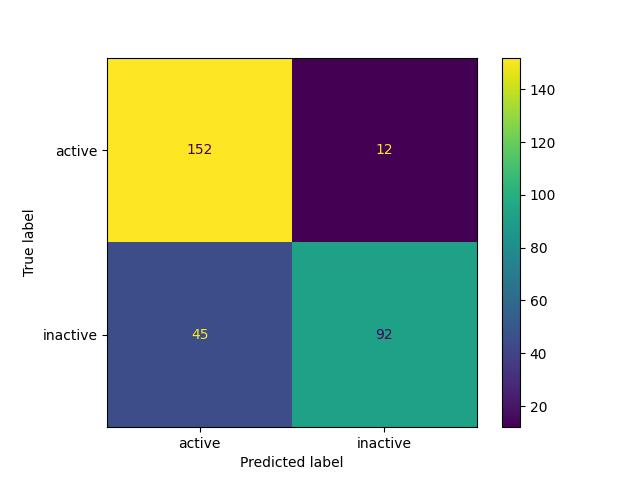
\includegraphics[height=8cm]{ache/baseline_rf_conf.jpg}
    \end{center}
\end{figure}
The confusion matrix for the baseline random forest model shows that it performs relatively well as the diagonal values(152, 92) are proportionally high
when compared to the rest of the values. The model is more likely to predict a false positive than it is predicting a false negative.  

\begin{figure}[H]
    \begin{center}
        \caption[]{SMOTE random forest confusion matrix}
        \label{fig:ache_smote_rf_conf}
        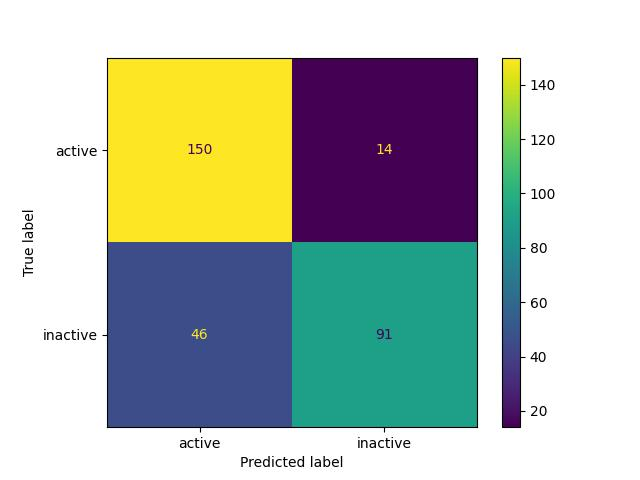
\includegraphics[height=8cm]{ache/fe_smote_rf_conf.jpg}
    \end{center}
\end{figure}
The matrix shows that the model is a fractionally less likely to predict a false negative when compared to \ref*{fig:ache_baseline_rf_conf}. However, the accuracy is marginally worse.  

\begin{figure}[H]
    \begin{center}
        \caption[]{Baseline random forest ROC curve}
        \label{fig:ache_baseline_rf_roc}
        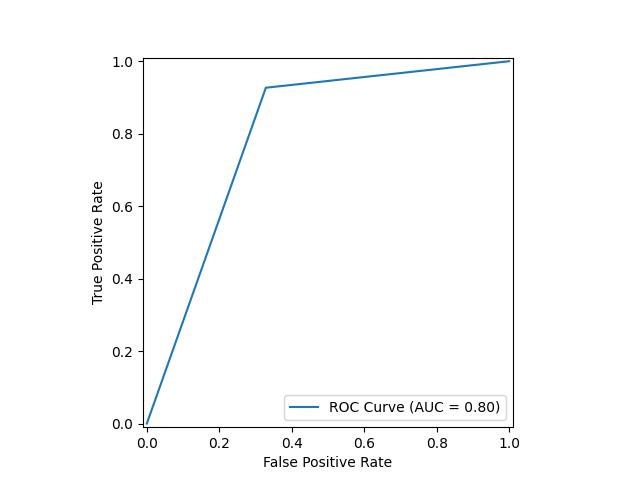
\includegraphics[height=8cm]{ache/baseline_rf_roc.jpg}
    \end{center}
\end{figure}
The ROC curve leans towards the top left corner, which indicates a good performance. It is closer to a perfect 1.0 than it is to the random threshold of 0.5.

\begin{figure}[H]
    \begin{center}
        \caption[]{SMOTE random forest ROC curve}
        \label{fig:ache_smote_rf_roc}
        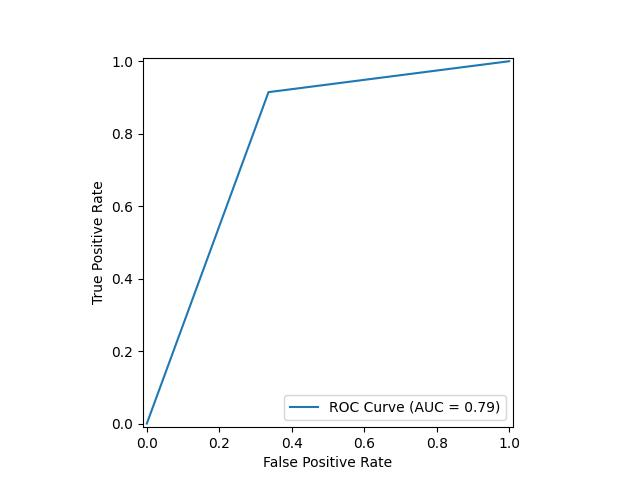
\includegraphics[height=8cm]{ache/fe_smote_rf_roc.jpg}
    \end{center}
\end{figure}
The appearance of the ROC curve signifies a good discriminative performance, although the AUC score of 0.79 indicates that the performance is not as good as \ref*{fig:ache_baseline_rf_roc}.

\subsection{Cyclooxygenase 1}
This table summarizes the performance of various machine learning algorithms on different test sets.
The top two performing configurations are visualized in ROC curves (see Figures \ref{fig:cox1_baseline_rf_roc} and \ref{fig:cox1_smote_rf_roc})
and confusion matrices (see Figures \ref{fig:cox1_baseline_rf_conf} and \ref{fig:cox1_smote_rf_conf}). Additionally, 
the scoring functions achieved an accuracy of 77.24\% on the test set.

\begin{table}[H]
    \begin{center}
        \caption{Cyclooxygenase 1 performance test-set}
        \begin{tabular}{lrrrrr}
            \toprule
            Name             & ACC    & FPR    & AUC    & EF     & REF     \\
            \midrule
            baseline\_rf     & 0.7724 & 0.0183 & 0.6344 & 2.8909 & 87.0968 \\
            fe\_smote\_rf    & 0.7628 & 0.0138 & 0.6155 & 2.9362 & 88.4615 \\
            fe\_rf\_per\_knn & 0.7019 & 0.0826 & 0.5598 & 1.7044 & 51.3514 \\
            baseline\_knn    & 0.6859 & 0.1147 & 0.5544 & 1.5153 & 45.6522 \\
            baseline\_nn     & 0.6827 & 0.0872 & 0.5309 & 1.4081 & 42.4242 \\
            fe\_smote\_nn    & 0.6827 & 0.1147 & 0.5490 & 1.4752 & 44.4444 \\
            fe\_rf\_mdi\_knn & 0.6250 & 0.1835 & 0.4987 & 0.9899 & 29.8246 \\
            \bottomrule
        \end{tabular}
    \end{center}
\end{table}

\begin{figure}[H]
    \begin{center}
        \caption[]{Baseline random forest confusion matrix}
        \label{fig:cox1_baseline_rf_conf}
        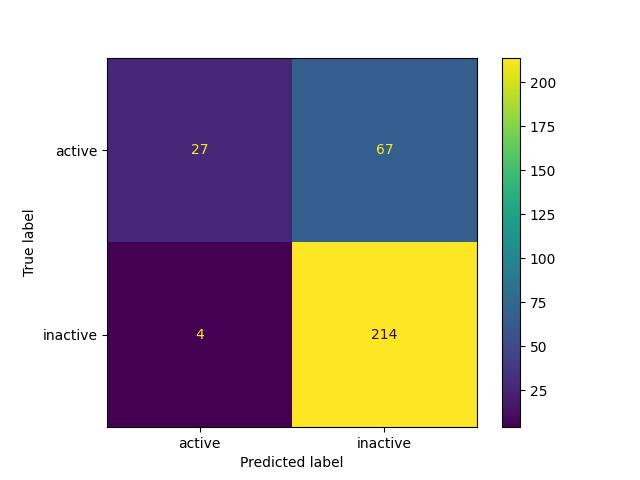
\includegraphics[height=8cm]{cox1/baseline_rf_conf.jpg}
    \end{center}
\end{figure}
This test-set contains more inactives than the test-set of the \acrshort*[]{ache} protein. This can be seen as the number of true negatives is far greater.  

\begin{figure}[H]
    \begin{center}
        \caption[]{SMOTE random forest confusion matrix}
        \label{fig:cox1_smote_rf_conf}
        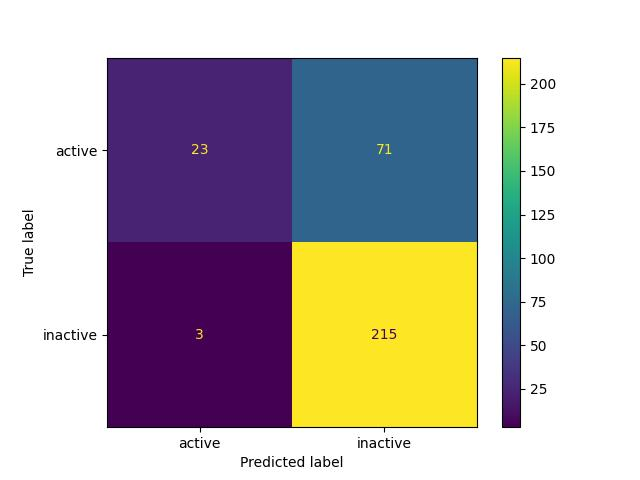
\includegraphics[height=8cm]{cox1/fe_smote_rf_conf.jpg}
    \end{center}
\end{figure}
The matrix shows that the model performed reasonably well with the diagonal values(23,215) being proportionally larger than the values of the other diagonal(3,71).

\begin{figure}[H]
    \begin{center}
        \caption[]{Baseline random forest ROC curve}
        \label{fig:cox1_baseline_rf_roc}
        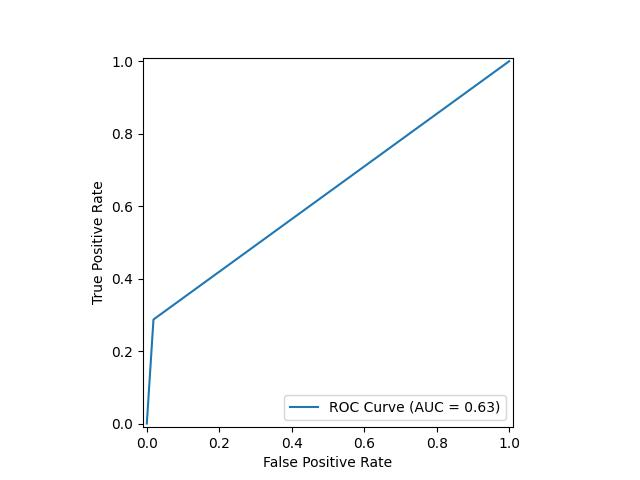
\includegraphics[height=8cm]{cox1/baseline_rf_roc.jpg}
    \end{center}

\end{figure}
The ROC curve indicates fair performance, as the AUC value is closer to 0.5 which would be a random estimator than it is to 1.0 which would indicate a perfect classifier.

\begin{figure}[H]
    \begin{center}
        \caption[]{SMOTE random forest ROC curve}
        \label{fig:cox1_smote_rf_roc}
        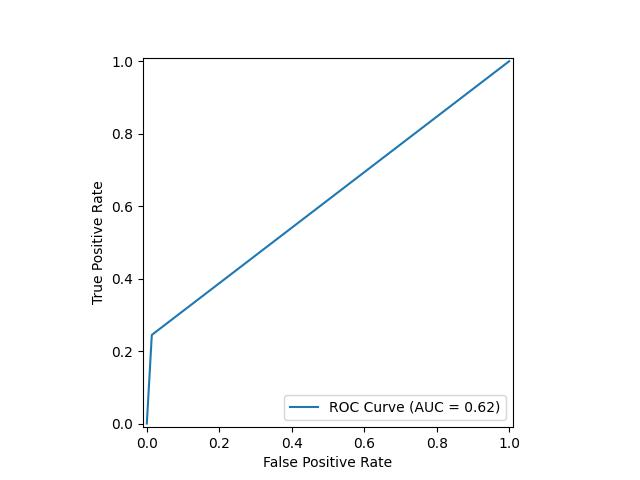
\includegraphics[height=8cm]{cox1/fe_smote_rf_roc.jpg}
    \end{center}
\end{figure}
The ROC curve indicates performance close to a random classifier. The AUC value is slightly worse than the value presented in \ref*{fig:ache_baseline_rf_roc}.

\subsection{Dipeptidyl peptidase IV}
Below the table representing the different results of the machine learning algorithms on the various test-sets can be found.
The confusion matrices for the top two performing configurations can be found at \ref{fig:dpp4_baseline_rf_roc} and \ref{fig:dpp4_smote_rf_roc}
respectively. The ROC curves can be found at \ref{fig:dpp4_baseline_rf_conf} and \ref{fig:dpp4_smote_rf_conf}.
The best scoring function was able to reach an accuracy of 77.21\% on the test-set.

\begin{table}[H]
    \begin{center}
        \caption{Dipeptidyl peptidase IV performance test-set}
        \begin{tabular}{lrrrrr}
            \toprule
            Name             & ACC    & FPR    & AUC    & EF     & REF     \\
            \midrule
            baseline\_rf     & 0.7721 & 0.2041 & 0.7730 & 1.5393 & 79.8387 \\
            fe\_smote\_rf    & 0.7662 & 0.2122 & 0.7670 & 1.5254 & 79.1165 \\
            fe\_rf\_per\_knn & 0.7112 & 0.3714 & 0.7082 & 1.3412 & 78.7879 \\
            baseline\_nn     & 0.6896 & 0.3347 & 0.6887 & 1.3425 & 71.2121 \\
            baseline\_knn    & 0.6896 & 0.3959 & 0.6865 & 1.3046 & 76.8939 \\
            fe\_smote\_nn    & 0.6896 & 0.3306 & 0.6889 & 1.3453 & 70.8333 \\
            fe\_rf\_mdi\_knn & 0.4892 & 0.5143 & 0.4891 & 0.9791 & 50.7812 \\
            \bottomrule
        \end{tabular}
    \end{center}
\end{table}

\begin{figure}[H]
    \begin{center}
        \caption[]{Baseline random forest confusion matrix}
        \label{fig:dpp4_baseline_rf_conf}
        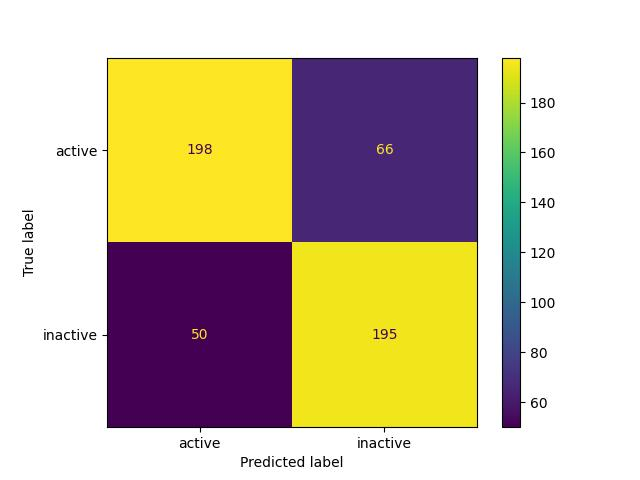
\includegraphics[height=8cm]{dpp4/baseline_rf_conf.jpg}
    \end{center}
\end{figure}
The confusion matrix indicates a very well-balanced dataset as there are nearly the same amount of actives as there are positives. The model is more likely to detect false negatives than it is to predict false positives.
\begin{figure}[H]
    \begin{center}
        \caption[]{SMOTE random forest confusion matrix}
        \label{fig:dpp4_smote_rf_conf}
        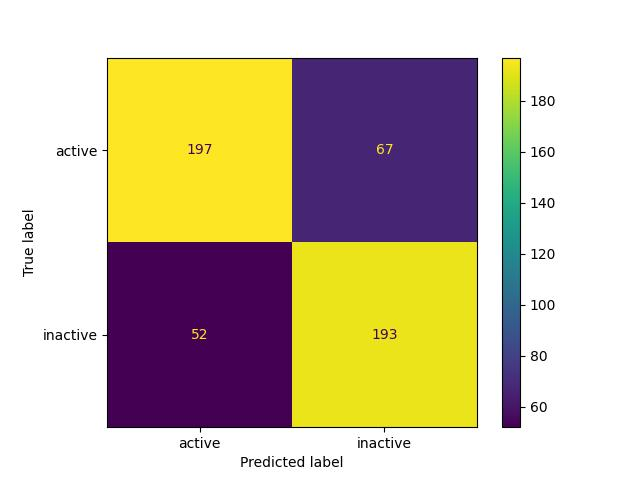
\includegraphics[height=8cm]{dpp4/fe_smote_rf_conf.jpg}
    \end{center}

\end{figure}
The confusion matrix describes a reasonably good model performance as the values in the diagonal(198, 195) far outweigh the other values.

\begin{figure}[H]
    \begin{center}
        \caption[]{Baseline random forest ROC curve}
        \label{fig:dpp4_baseline_rf_roc}
        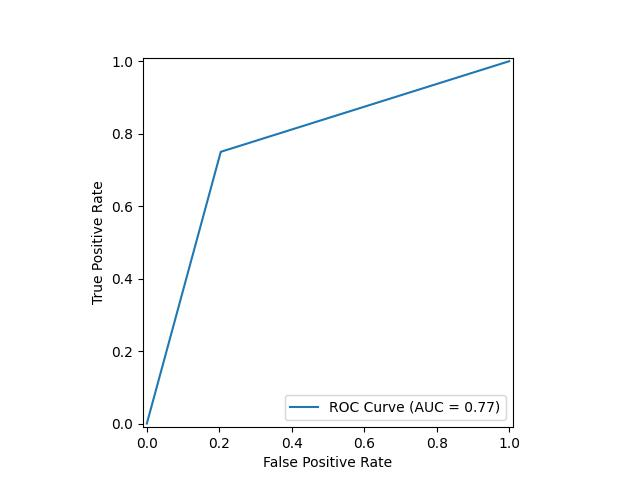
\includegraphics[height=8cm]{dpp4/baseline_rf_roc.jpg}
    \end{center}
\end{figure}
The model is performing well at classifying between positive and negative classes. The AUC score is 0.77 which further indicates good performance.

\begin{figure}[H]
    \begin{center}
        \caption[]{SMOTE random forest ROC curve}
        \label{fig:dpp4_smote_rf_roc}
        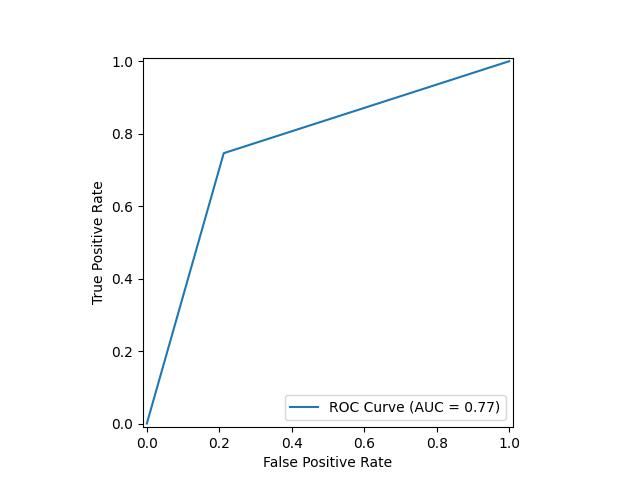
\includegraphics[height=8cm]{dpp4/fe_smote_rf_roc.jpg}
    \end{center}
\end{figure}
The ROC curve suggests that the performance of the random forest doesn't change with the introduction of SMOTE.

\subsection{Monoamine oxidase B}
This table summarizes the performance of various machine learning algorithms across different test sets.
The top two configurations, visualized in ROC curves (see Figures \ref{fig:maob_baseline_rf_roc} and \ref{fig:maob_fe_rf_per_knn_roc}),
are further analyzed in confusion matrices (see Figures \ref{fig:maob_baseline_rf_conf} and \ref{fig:maob_fe_rf_per_knn_conf}). 
The best scoring function achieved an accuracy of 75.98\% on the test set.

\begin{table}[H]
    \begin{center}
        \caption{Monoamine oxidase B performance test-set}
        \begin{tabular}{lrrrrr}
            \toprule
            Name             & ACC    & FPR    & AUC    & EF     & REF     \\
            \midrule
            baseline\_rf     & 0.7589 & 0.1389 & 0.7181 & 1.9515 & 69.6970 \\
            fe\_rf\_per\_knn & 0.7054 & 0.1944 & 0.6653 & 1.6800 & 60.0000 \\
            fe\_smote\_rf    & 0.7054 & 0.1944 & 0.6653 & 1.6800 & 60.0000 \\
            baseline\_nn     & 0.6964 & 0.1806 & 0.6472 & 1.6625 & 59.3750 \\
            baseline\_knn    & 0.6786 & 0.1667 & 0.6167 & 1.6000 & 57.1429 \\
            fe\_smote\_nn    & 0.6696 & 0.2222 & 0.6264 & 1.5200 & 54.2857 \\
            fe\_rf\_mdi\_knn & 0.5804 & 0.3333 & 0.5458 & 1.1610 & 42.5000 \\
            \bottomrule
        \end{tabular}
    \end{center}
\end{table}

\begin{figure}[H]
    \begin{center}
        \caption[]{Baseline random forest confusion matrix}
        \label{fig:maob_baseline_rf_conf}
        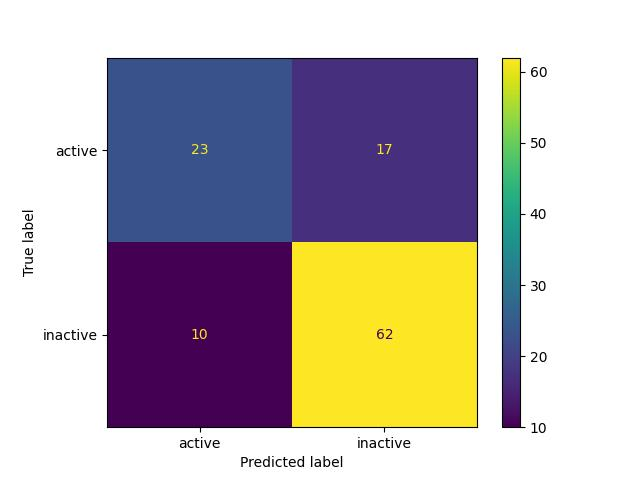
\includegraphics[height=8cm]{maob/baseline_rf_conf.jpg}
    \end{center}
\end{figure}
The confusion matrix shows, that the majority of samples in the test-set is inactive. The number of false positives is smaller, than the number of false negatives. 
\begin{figure}[H]
    \begin{center}
        \caption[]{Feature engineering permutation importance confusion matrix}
        \label{fig:maob_fe_rf_per_knn_conf}
        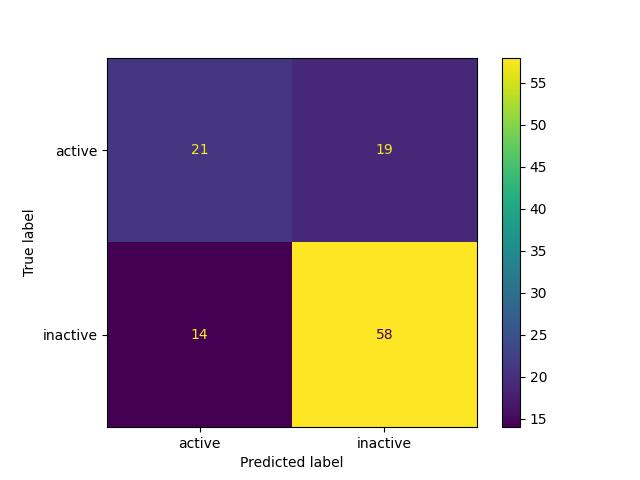
\includegraphics[height=8cm]{maob/fe_rf_per_knn_conf.jpg}
    \end{center}

\end{figure}
The model is reasonably accurate, as there are 21 true positives and 58 true negatives. Overall it performs slightly worse than the baseline random forest.
\begin{figure}[H]
    \begin{center}
        \caption[]{Baseline random forest ROC curve}
        \label{fig:maob_baseline_rf_roc}
        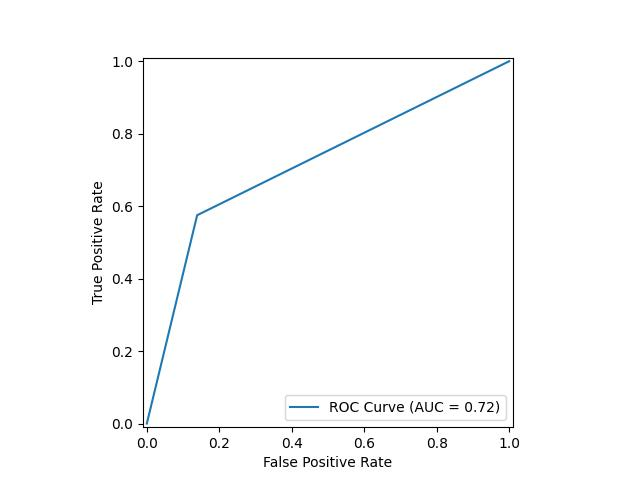
\includegraphics[height=8cm]{maob/baseline_rf_roc.jpg}
    \end{center}

\end{figure}
Achieving an AUC of 0.72, the model demonstrates strong ability to distinguish between positive and negative instances.

\begin{figure}[H]
    \begin{center}
        \caption[]{Feature engineering permutation importance ROC curve}
        \label{fig:maob_fe_rf_per_knn_roc}
        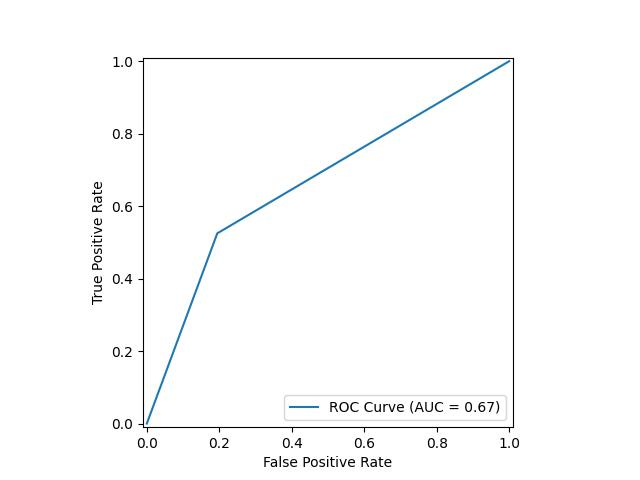
\includegraphics[height=8cm]{maob/fe_rf_per_knn_roc.jpg}
    \end{center}
\end{figure}
The ROC curve suggests good discrimination between classes, but the AUC score of 0.67 indicates that it falls short of the reference value of \ref*{fig:maob_baseline_rf_roc}.
\subsection{Soluble epoxide hydrolase}
This table compares the performance of various machine learning algorithms across different test sets.
The two most effective configurations (visualized in confusion matrices: figures \ref{fig:maob_baseline_rf_conf} and \ref{fig:maob_fe_rf_per_knn_conf}) 
are further analyzed in ROC curves (figures \ref{fig:maob_baseline_rf_roc} and \ref{fig:maob_fe_rf_per_knn_roc}). 
Overall, the scoring functions achieved an accuracy of 80.00\% on the test set.

\begin{table}[H]
    \begin{center}
        \caption{Soluble epoxide hydrolase performance test-set}
        \begin{tabular}{lrrrrr}
            \toprule
            Name             & ACC    & FPR    & AUC    & EF     & REF      \\
            \midrule
            fe\_rf\_per\_knn & 0.8000 & 0.0667 & 0.6667 & 2.6667 & 66.6667  \\
            baseline\_nn     & 0.7833 & 0.0667 & 0.6333 & 2.5000 & 62.5000  \\
            baseline\_rf     & 0.7667 & 0.0000 & 0.5333 & 4.0000 & 100.0000 \\
            fe\_smote\_rf    & 0.7667 & 0.0000 & 0.5333 & 4.0000 & 100.0000 \\
            baseline\_knn    & 0.7333 & 0.0222 & 0.4889 & 0.0000 & 0.0000   \\
            fe\_rf\_mdi\_knn & 0.7000 & 0.1333 & 0.5333 & 1.3333 & 33.3333  \\
            fe\_smote\_nn    & 0.7000 & 0.0889 & 0.4889 & 0.8000 & 20.0000  \\
            \bottomrule
        \end{tabular}
    \end{center}
\end{table}

\begin{figure}[H]
    \begin{center}
        \caption[]{Feature engineering permutation importance confusion matrix for \acrshort*[]{knn}}
        \label{fig:seh_fe_rf_per_knn_conf}
        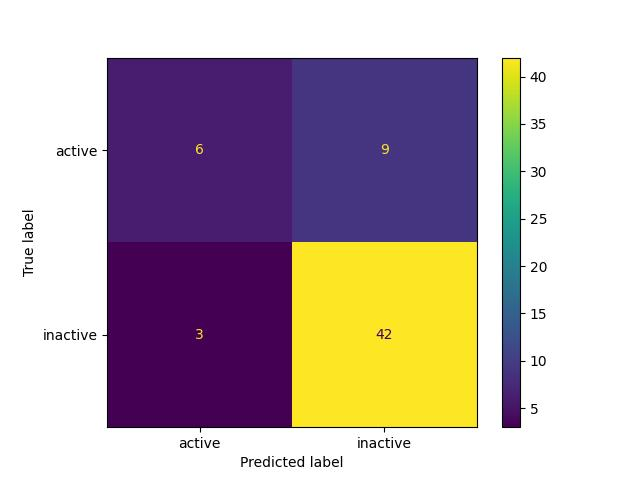
\includegraphics[height=8cm]{seh/fe_rf_per_knn_conf.jpg}
    \end{center}
\end{figure}
The confusion matrix indicates a very small test-set. In addition to that the dataset is also very imbalanced.

\begin{figure}[H]
    \begin{center}
        \caption[]{Baseline neural network confusion matrix}
        \label{fig:seh_baseline_nn_conf}
        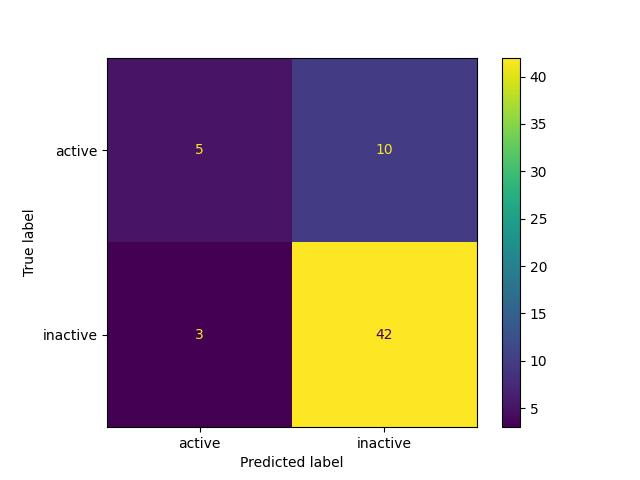
\includegraphics[height=8cm]{seh/baseline_nn_conf.jpg}
    \end{center}

\end{figure}
The proportionally high values in the diagonal(5, 42) signify good overall performance. Although the \acrshort*[]{knn} performance of \ref*{fig:seh_fe_rf_per_knn_conf} is marginally better.
\begin{figure}[H]
    \begin{center}
        \caption[]{Feature engineering permutation importance ROC curve}
        \label{fig:seh_fe_rf_per_knn_roc}
        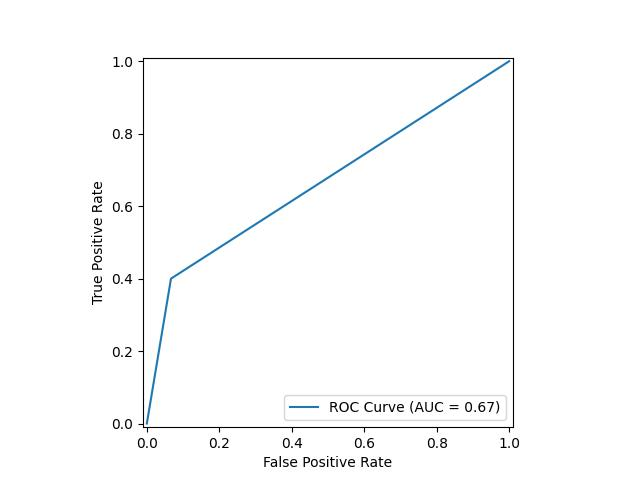
\includegraphics[height=8cm]{seh/fe_rf_per_knn_roc.jpg}
    \end{center}

\end{figure}
An AUC of 0.67 demonstrates the model's ability to differentiate between positive and negative examples. Overall the performance is close to a random classifier.

\begin{figure}[H]
    \begin{center}
        \caption[]{Baseline neural network ROC curve}
        \label{fig:seh_baseline_nn_roc}
        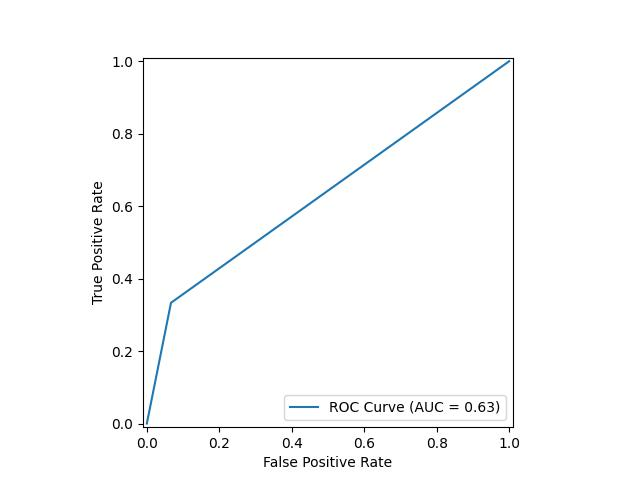
\includegraphics[height=8cm]{seh/baseline_nn_roc.jpg}
    \end{center}
\end{figure}
The ROC curve demonstrates only fair performance as it is much closer to a random classifier than it is to a perfect classifier which would be a 1.0 AUC.

\section{Performance Overview -- Comparing ML-approaches → maybe use median instead of avg ask MICHA}
Compare performance of overall ml approaches.
\chapter{Discussion}
\label{cha:Discussion}

The overall performance of the models compares well to the scoring functions introduced in \cite[]{Birklbauer2021}.
The following table represents the results for the \acrshort*[]{ache} protein in \cite[]{Birklbauer2021}:
\begin{figure}[H]
    \begin{center}
        \caption[]{Scoring results for ACHE Birklbauer}
        \label{fig:ache_birklbauer}
        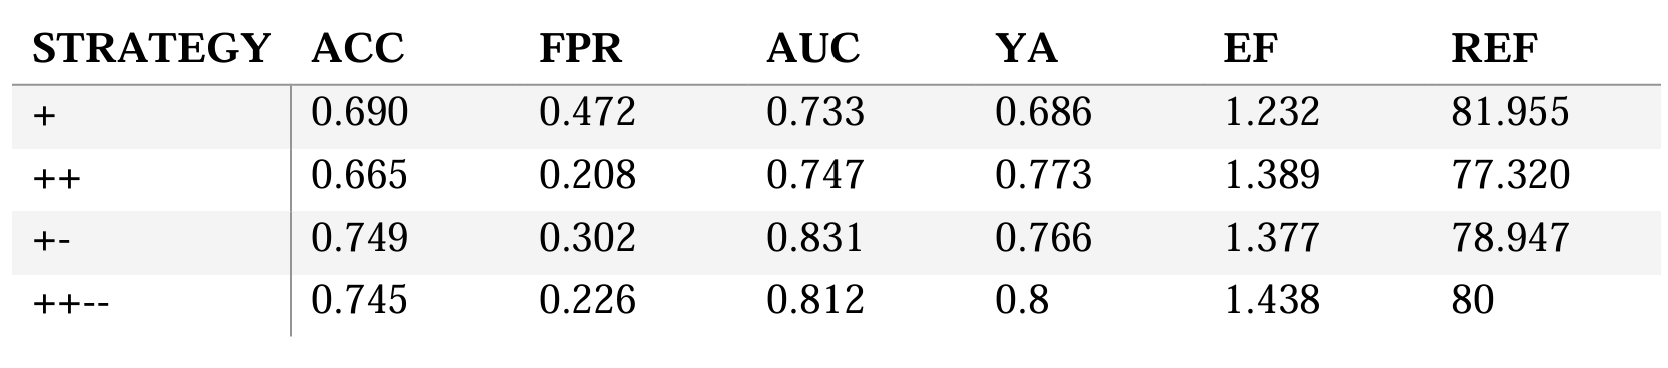
\includegraphics[width=14cm]{discussion/Birklbauer_ACHE.png}
    \end{center}
\end{figure}
The following results were achieved for the \acrshort*[]{ache} protein using the methods proposed in this thesis:
\begin{table}[H]
    \begin{center}
        \caption{Acetylcholinesterase performance test-set}
        \begin{tabular}{lrrrrrr}
            \toprule
            Name             & ACC    & FPR    & AUC    & YA     & EF     & REF     \\
            \midrule
            baseline\_rf     & 0.8106 & 0.3285 & 0.7992 & 0.7716 & 1.4161 & 92.6829 \\
            fe\_smote\_rf    & 0.8007 & 0.3358 & 0.7894 & 0.7653 & 1.4046 & 91.4634 \\
            fe\_smote\_nn    & 0.7708 & 0.2993 & 0.7650 & 0.7684 & 1.4102 & 82.9268 \\
            baseline\_nn     & 0.7674 & 0.2920 & 0.7626 & 0.7701 & 1.4134 & 81.7073 \\
            fe\_rf\_per\_knn & 0.7575 & 0.4307 & 0.7420 & 0.7177 & 1.3172 & 91.4634 \\
            baseline\_knn    & 0.6844 & 0.5766 & 0.6629 & 0.6520 & 1.1966 & 90.2439 \\
            fe\_rf\_mdi\_knn & 0.5515 & 0.4307 & 0.5530 & 0.5986 & 1.0987 & 59.8639 \\
            \bottomrule
        \end{tabular}
    \end{center}
\end{table}

The comparison between the two tables underlines the performance improvements of the machine learning approaches
over the simple scoring functions introduced in \cite[]{Birklbauer2021}.
Generally the improvements in \acrshort*[]{acc} and \acrshort*[]{ref} are most notable.
The improvements in the \acrshort*[]{ref} metric are of particular interest, as there is less money spent on investigating false positive compounds.
Similar performance benefits can be observed for the other protein complexes.

\section{Improvements and outlook}
This thesis serves as a proof of concept for the applicability of machine learning models in combination with feature engineering for protein docking, as the achieved results 
are more accurate than those achieved using traditional approaches.

However, the machine learning approaches for protein docking where implemented using standard approaches and models. 
Through the use of more problem-tailored algorithmic methods the quality of the results will probably increase. Additionally, only a small sample 
of protein-ligand complexes was researched for this thesis. The machine learning methods proposed within this thesis need to be evaluated on a larger subset of 
protein-ligand compounds to determine whether machine learning is a viable approach for protein docking.


%%%-----------------------------------------------------------------------------
\appendix                                                             % Appendix 
%%%-----------------------------------------------------------------------------

\chapter{Technical Details}
\label{app:TechnicalDetails}



 % Technical supplements
\chapter{Supplementary Materials}
\label{app:materials}


List of supplementary data submitted to the degree-granting institution for archival storage
(in ZIP format).

% Use this as an example only, adapt the structure to your requirements!

\section{PDF Files}
\begin{FileList}{/}
\fitem{thesis.pdf} Master/Bachelor thesis (complete document)
\end{FileList}

\section{Media Files}
\begin{FileList}{/media}
\fitem{*.ai, *.pdf} Adobe Illustrator files
\fitem{*.jpg, *.png} raster images
\fitem{*.mp3} audio files
\fitem{*.mp4} video files
\end{FileList}


\section{Online Sources (PDF Captures)}
\begin{FileList}{/online-sources}
\fitem{Reliquienschrein-Wikipedia.pdf} \citenobr{WikiReliquienschrein2022}
\end{FileList}




 % Contents of the CD-ROM/DVD
\chapter{Questionnaire}
\label{app:Questionnaire}





 % Chronological list of changes
\chapter{\latex Source Code}
\label{app:SourceCode}

 % Source text of this document

%%%-----------------------------------------------------------------------------
\backmatter                           % Back part (bibliography, glossary, etc.)
%%%-----------------------------------------------------------------------------

\MakeBibliography % References

%%%-----------------------------------------------------------------------------
% Special page for checking print size
%%%-----------------------------------------------------------------------------

\chapter*{Check Final Print Size}

\begin{center}
{\Large --- Check final print size! ---}

\bigskip

\calibrationbox{100}{50} % width/height of box in mm

\bigskip

{\Large --- Remove this page after printing! ---}

\end{center}



%%%-----------------------------------------------------------------------------
\end{document}
%%%-----------------------------------------------------------------------------
